\documentclass[11pt, oneside]{article} 
\usepackage{geometry}
\geometry{letterpaper} 
\usepackage{graphicx}
	
\usepackage{amssymb}
\usepackage{amsmath}
\usepackage{parskip}
\usepackage{color}
\usepackage{hyperref}

\graphicspath{{/Users/telliott_admin/Dropbox/Tex/png/}}
% \begin{center} 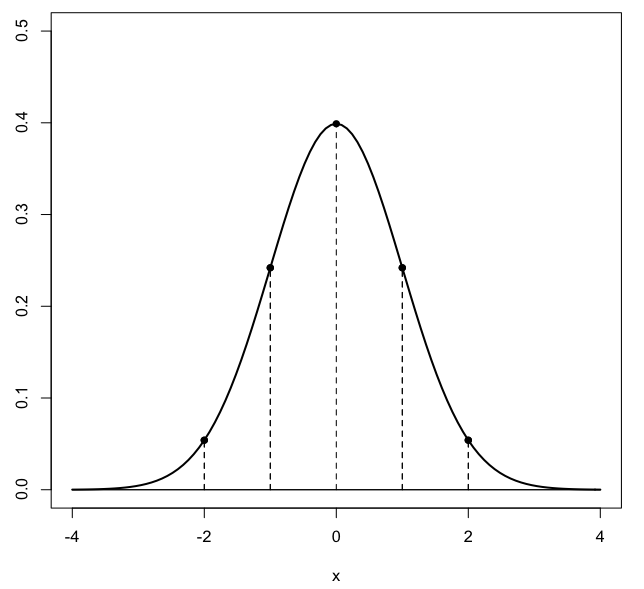
\includegraphics [scale=0.4] {gauss3.png} \end{center}

%break
\title{Polar ellipse}
\date{}

\begin{document}
\maketitle
\Large
\label{sec:Polar_ellipse}

We usually talk about the ellipse as the set of points whose combined distance to two foci is a constant.  And typically, we place the origin halfway between the two foci.

We can also use one of the foci together with its corresponding directrix.
\begin{center} 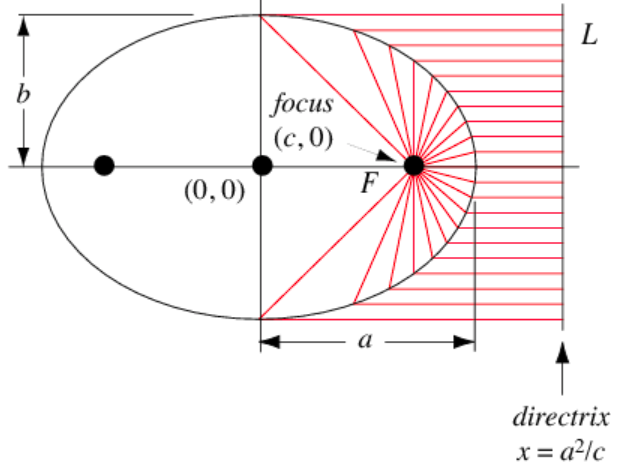
\includegraphics [scale=0.4] {ellipse_directrix.png} \end{center}

\url{http://mathworld.wolfram.com/Ellipse.html}

Points on the ellipse have the following property:  the distance from the focus is \emph{proportional} to the horizontal distance from the directrix, where that ratio is less than $1$.  

Let $e$ be the ratio.  I've chosen to use $e$ here for reasons that should be clear in a minute. 

Consider the point $P = (a,0)$.  The distance from the focus to $P$ is $a - c$.  

Let $d$ be the total distance from the origin to the directrix.  The distance from the directrix to $P$ is $d-a$.

The ratio is
\[ e = \frac{a - c}{d - a} \]

On the other hand, consider the point $Q = (0,b)$.  The distance from the focus is $\sqrt{b^2 + c^2}$ by Pythagoras and the distance from $Q$ to the directrix is the total distance $d$.  

However, we have seen before that the distance of $Q$ from the focus is also $a$. (See \hyperref[sec:Ellipse_geometry]{\textbf{here}}, this is how we obtain $b^2 + c^2 = a^2$).  

So the ratio is
\[ e = \frac{a}{d} = \frac{a - c}{d - a}  \]

Solving for $d$:
\[ d(a - c) = a(d - a) \]
\[ cd = a^2 \]
\[ d = \frac{a^2}{c} \]

From above, the ratio $e$ is
\[ e = \frac{a}{d} = \frac{a \cdot c}{a^2} = \frac{c}{a} \]
\[ ae = c \]
We have previously used this as the definition of the eccentricity, the fraction of $a$ that the focus moves out from the origin.

Hence, working with the equation we solved for $d$ above
\[ d = \frac{a^2}{c} \]
\[ = \frac{a^2}{ae} = \frac{a}{e} \]
So we have the parallel equations:
\[ a = ed \]
\[ c = ea = e^2 d \] 

Let $p$ be the distance from the focus to the directrix.
\[ p = d - c \]
\[ = \frac{a^2}{c} - c \]
\[ = \frac{a^2 - c^2}{c} \]
\[ = \frac{b^2}{c} \]

In a way this definition of $p$ is analogous to that for $d$
\[ d = \frac{a^2}{c}, \ \ \ \  p = \frac{b^2}{c} \]

Putting $p$ in terms of $e$
\[ p = \frac{a^2 - c^2}{c} \]
\[ = \frac{a^2 - a^2e^2}{ae} \]
\[ = \frac{a(1-e^2)}{e} \]
so
\[ ep = a(1-e^2) \]

If you allow me to shift to another picture (from Kline):
\begin{center} 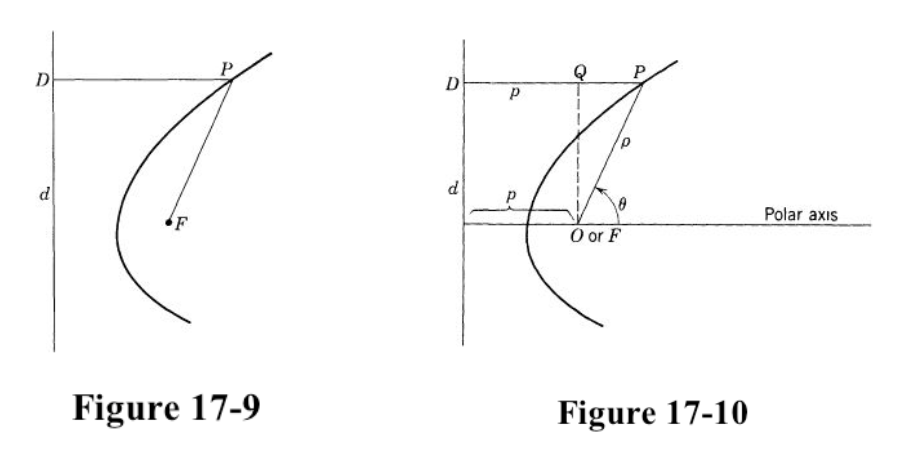
\includegraphics [scale=0.5] {Kline_17_10.png} \end{center}

In the left panel we have a parabola, and on the right, an ellipse.  We have said that for a parabola, the distance from point $P$ on the curve to the focus, $PF$, is equal to the distance from the point to the directrix, $PD$.  For an ellipse, the relationship is almost the same, $PF$ is smaller by a factor which we call $e$.

As we stated, $p$ has been defined to be the distance from the directrix to the focus.

We now place the origin at the focus.  In the figure, the distance $PF$ is the "radius" $r$ (somewhat confusingly labeled as $\rho$ in the diagram) and $\theta$ is the angle that $r$ makes with the positive $x$-axis, as usual.  With this setup, writing the equation of the ellipse in polar coordinates is almost trivial.

We have
\[ x = p + r \cos \theta \]
\[ y = r \sin \theta \]

As Kline says, we wish to express in these coordinates the geometric condition
\[ \frac{PF}{PD} = e \]
But $PF = r$ and
\[ PD = x + p = r \cos \theta + p \]
So
\[ e = \frac{r}{ r \cos \theta + p} \]

Solve for $r$:
\[ \frac{1}{e} = \cos \theta + \frac{p}{r} \]
\[ 1 - e \cos \theta =  \frac{ep}{r} \]
\[ r = \frac{ep}{1 - e \cos \theta} \]

We obtain a standard equation for an ellipse in polar coordinates.  If you want the long axis in the $y$ direction, substitute $\sin \theta$ for $\cos \theta$.  The minus sign makes it open to the right, or to put it another way, we have chosen the left focus as the origin.  Because of the translation, to convert back to an ellipse centered on the origin, we need $x' = x - c$.

This equation will come in handy when we talk about Kepler's laws for planetary orbits.

\subsection*{back to Cartesian coordinates}
In order to convince ourselves that this equation is correct, we should be able to convert the polar form back to $xy$-coordinates.  Let's massage the equations:

Start with
\[ r = \frac{ep}{1 - e \cos \theta} \]
We have $x/r = \cos \theta$ so
\[ r = \frac{ep}{1 - ex/r} \]
\[ r (1 - ex/r) = ep \]
\[ r - ex = ep \]
\[ r = e( p + x) \]

As usual, go back to $x$ and $y$ by squaring $r$
\[ r^2 = e^2 (p + x)^2 \]
\[ x^2 + y^2 = e^2( p^2 + 2px + x^2) \]
\[ (1-e^2) x^2 - 2pe^2 x + y^2 = e^2 p^2 \]

Our first task is to complete the square for $x$.  Recall that 
\[ ep = a(1-e^2) \]
\[ 1 - e^2 = \frac{ep}{a} \]
so
\[ (1-e^2) x^2 - 2pe^2 x + y^2 = e^2 p^2 \]
becomes
\[ \frac{ep}{a} x^2 - 2pe^2 x + y^2 = e^2 p^2 \]
\[ x^2 - 2ae x + \frac{ay^2}{ep} = aep \]
but $ae = c$
\[ x^2 - 2c x + \frac{ay^2}{ep} = cp \]
Complete the square:
\[ x^2 - 2c x + c^2 + \frac{ay^2}{ep} = cp + c^2 \]
\[ (x-c)^2 + \frac{ay^2}{ep} = cp + c^2 \]
Our ellipse is re-centered.  Now we just have to work out the details.

Use these identities:
\[ p = b^2/c = b^2/ae \] 
and thus 
\[ pe = b^2/a \] 
and
\[ cp = b^2 \]

We have
\[ (x-c)^2 + \frac{ay^2}{ep} = cp + c^2 \]
which becomes
\[ (x-c)^2 + a^2 \frac{y^2}{b^2} = b^2 + c^2 \]
but $a^2 = b^2 + c^2$ so
\[ (x-c)^2 + a^2 \frac{y^2}{b^2} = a^2 \]
\[ \frac{(x-c)^2}{a^2} + \frac{y^2}{b^2} = 1 \]
Got there!

\subsection*{Another version}
I worked the problem a different way, substituting in familiar quantities and then completing the square.  I'm not sure which one is simpler.

Repeat the useful identities:
\[ a^2 = b^2 + c^2 \]

\[ a = ed , \ \ \ \ c = ea = e^2 d \]
\[ d = \frac{a}{e} = \frac{a^2}{c} \]

\[ p = d - c = \frac{a^2}{c} - \frac{c^2}{c} = \frac{b^2}{c}  \]
The polar equation for the ellipse is:
\[ r = \frac{pe}{1 - e \cos \theta} \]
Since $x/r = \cos \theta$:
\[ r = \frac{pe}{1 - ex/r} \]
\[ r - ex = pe \]
\[ r = pe + ex \]
Continuing the journey back to Cartesian coordinates we substitute for $r^2$ (as always):
\[ r^2 = x^2 + y^2 = e^2(p^2 + 2px + x^2) \]
\[ (1-e^2)x^2 - 2pe^2x + y^2 = p^2 e^2 \]

I admit it, this looks like a mess.  The goal is to complete the square on $x$, and the question is whether to do that directly or try to simplify first.  We opt for the latter
\[ 1 - e^2 = 1 - \frac{c^2}{a^2} = \frac{b^2}{a^2} \]
\[ pe^2 = \frac{b^2}{c} \cdot \frac{c^2}{a^2} = \frac{b^2}{a^2} \ c \]
Substitute into the expanded equation from above
\[ (1-e^2)x^2 - 2pe^2x + y^2 = p^2 e^2 \]
\[  \frac{b^2}{a^2} x^2 - 2 \frac{b^2}{a^2} \ cx + y^2 = p^2 e^2 \]
\[ \frac{1}{a^2} (x^2 - 2cx) + \frac{y^2}{b^2} = \frac{p^2 e^2}{b^2} \]
And we're definitely on the right track because adding $c^2$ inside the parentheses on the left gives
\[ \frac{1}{a^2} (x-c)^2 +  \frac{y^2}{b^2}  \]
We have the ellipse with the origin at one focus, which is correct.  All that remains is to figure out the constant.  We add $c^2/a^2  = e^2$ to the right-hand side, substituting for $e^2$ in the original term:
\[ \frac{p^2 c^2}{b^2 a^2} + \frac{c^2}{a^2}  \]
and substitute for $p^2 = b^4/c^2$
\[ = \frac{b^2}{a^2} + \frac{c^2}{a^2} = \frac{b^2 + c^2}{a^2} = 1 \]
We're done!

\end{document}